\documentclass[UTF8,11pt]{ctexart}
\usepackage[margin=1in]{geometry}
\usepackage{amsmath,amssymb,booktabs,array,longtable,graphicx,xurl}
\usepackage[hidelinks]{hyperref}
\usepackage{tikz,placeins,needspace}
\usetikzlibrary{arrows.meta}
\setlength{\emergencystretch}{3em}
\newcommand{\R}{\mathbb{R}}
\newcommand{\ES}{\operatorname{ES}}
\newcommand{\supp}[1]{\href{supplement.pdf\##1}{科学补充材料}}
\newcommand{\audit}[1]{\href{audit-notes.pdf\##1}{审查记录}}
% Generated from original public aggregate values; no inference.
\newcommand{\FullES}{477.85}
\newcommand{\InertialES}{824.73}
\newcommand{\FullFDE}{1326.09}
\newcommand{\FullADE}{636.11}
\newcommand{\InertialDelta}{-346.87}
\newcommand{\PointRowFull}{Full & 73.77 & 332.31 & 812.26 & 1326.09\\}
\newcommand{\PointRowGMM}{GMM & 71.92 & 323.79 & 792.99 & 1299.11\\}
\newcommand{\PointRowdtThreeHundred}{dt300 & 75.88 & 340.10 & 825.76 & 1335.73\\}
\newcommand{\PointRowInertial}{Inertial & 31.17 & 237.93 & 934.03 & 2095.78\\}

\author{}
\date{公开审阅修订稿，2026年10月9日；署名待确认}

\title{审查记录：证据版本与执行历史}
\begin{document}\maketitle
\section{记录的阅读范围}
科学算术、执行终态、文稿编辑与人类验收分别判断。
2026年10月9日修订保留原结果、协议与五项失败；逐单元迁移见
\path{revision46-source-migration.json}，改前中英逐字源稿为
\texttt{historical-main-v1.tex}。历史等待计数和旧声明布尔值是带日期快照，
不是今日队列。没有重跑失败、重复成功审计，或新增拟合、预测、种子、bootstrap预算。

计数为46个独特记录哈希块、58个复用起点--模式案例，不是58个独立记录。
历史\texttt{closed\_blocks}、\texttt{support\_blocks}等字段指程序组，
原JSON语义不擅自升级为参与者身份。11,368评分槽含11,363成功与五失败。
必需失败使四个家族／模式单元不可用，包括两个主地形家族。
缺异常栈、资源／退出记录时，失败根因未知；控制器摘要不证明数值发散、OOM、
精确超时或物理断电。公开记录不含私有机器路径或原始路线。

\section{复现层次与保留决定}
稿件构建、保存汇总重绘、固定随机流统计复算、权限内原始输出审计是不同层次。
原独立审计与后续完整公开固定流复算的报告和绑定见
\texttt{qualification-v1}、\texttt{public-paired-replay-v1}、\texttt{final-results-v1}。
原42问题身份与标准保留在\path{review-response-v1.json}，
\path{review-current-v2.md}保留随后作者分类，不是审查人接受。
本次46项记录应区分编辑、自动核查、科学缺口与真实权限／验收。
编辑完成不等于科学限制消失，也不等于论文已被接受。

\section{必须真实确认的发表选择}
不推断作者、机构、贡献、利益声明或伦理编号。
路线公开与各地图图层再分发需要分别确认；未确认前PR仅含已有公开汇总和匿名复算记录。
本地真实地图审阅材料不自动上传。
本次论文修改请求授权交付PR，不授权虚构审查通过或新增科学重跑。

\section{保留的版本、成本与执行材料}
下列单元保留详细旧记录，当前闭合状态以其中审计更新为准，
旧排队数字只描述其历史捕获时点。
\section{地形消融结果}
\label{sec:terrain-results}\hypertarget{sec:terrain-results}{}
登记完整家族终局为不可用，不是等待剩余预测：保留必需失败使总体／LOO及LIO推断
按原规则无法成立，不是零效应或等价。整体比较链接 \texttt{terrain:all-vs-base}，四组链接
\texttt{terrain:road}、\texttt{terrain:river}、\texttt{terrain:worldcover}、\texttt{terrain:surface}。
每组报告主要完整模型移除、支持性基线加入、输入维度、覆盖与缺失、配对效应与区间、
稳定性、资格、裁定、成本和局限。

整体比较回答组合是否改善历史基线；LOO 回答组在完整模型中的增量价值；LIO 回答组单独加入
基线是否提供信息。三层证据共同报告，不能事后挑选更有利比较。六块次要模式描述初始化
敏感性，但不赋予次要因素裁定。

表~\ref{tab:terminal-score-inventory} 的闭合评分清单已包含全部计划地形槽。
在 46 个主要记录哈希块、五个固定预测种子上，整体/LOO 家族所需的六个配置
共 1380 行：1379 成功、1 失败、0 缺项；支持性 LIO 家族所需的五个配置
共 1150 行：1148 成功、2 失败、0 缺项。两者共享全部 230 行基线，
并集为 2300 份不同的主要地形预测，其中 2297 成功、3 项保留失败，
不是 2530 份独立预测或独立观测。
仅计数投影 \texttt{terrain-family-completeness-v1.json} 使用同一闭合评分索引与原登记比较成员。
第~\ref{sec:execution-coverage} 节原先的 160/131 行缺项作为有日期的历史快照保留，
不再代表当前未完成预测数量。

尽管执行已经终结，原完整配对规则仍使两个主要模式地形家族整体不可用：
全地形失败影响整体及四项 LOO 比较，LIO 失败影响支持性家族。
本工作不从成功交集估计地形效应或区间。因此，现有结果不能确立道路、河流、
地表覆盖或坡面因素相比历史基线有益、有害或等效。
现已完成的辅助试验或保存输出审计，本身不会替换失败预测或恢复这些比较。
闭合计数仅描述保存的状态，不等于独立原输出审计或最终证据卡片验收。

\paragraph{执行终结与可用推断。}
\label{sec:terminal-failures}\hypertarget{sec:terminal-failures}{}
当前不自动重试的策略下，全部原科学预测均已终结，已经记录的失败仍予保留。
登记的比较家族只要有任何必需行失败，即使全部计划任务都已有终结处置，
该家族仍不可用于完整配对推断。因此，执行完成与配对推断可用是不同条件。
本工作不会将失败补为零、删除失败行或重新定义登记家族来制造结果。
比较不可用既不代表效应为零，也不是等效性的证据。

\paragraph{五项失败实际证明了什么。}
表~\ref{tab:retained-failures} 列明保留的配置及预测种子。
原检查点包含三项通用控制器中断，以及两项没有完成回复的在途保留。
本次检查的前后两个检查点根目录均没有这五项的逐项回复文件；
这只是对两个指定位置的观察，不声称搜索过全部可能的历史日志。
最后一次串行请求明确对应 \texttt{lio-river}，关闭记录证明其所属进程树活动进程为零。
另两项绑定原先不同的并发路线，各保留180秒成本。
保留秒数是保守记账，不是预测实测耗时，也不能证明180秒超时。

\begin{table}[htbp]
\centering\small
\caption{五项保留的执行中断。标签仅用于本说明，不以成功子集替代失败输出。}
\label{tab:retained-failures}\hypertarget{tab:retained-failures}{}
\begin{tabular}{llll}
\toprule
标签 & 配置 & 起点模式 & 预测种子\\
\midrule
F01 & \texttt{arm-06/dt30} & \texttt{known\_velocity} & 20260814\\
F02 & \texttt{arm-03/single\_gaussian} & \texttt{known\_velocity} & 20260817\\
F03 & \texttt{lio-river} & \texttt{causal\_prefix} & 20260817\\
F04 & \texttt{all-terrain} & \texttt{causal\_prefix} & 20260815\\
F05 & \texttt{lio-road} & \texttt{causal\_prefix} & 20260814\\
\bottomrule
\end{tabular}
\end{table}

方法阶段的同期运行摘要记录了Windows替换共享请求文件失败，
但没有分别提供F01和F02的异常栈。另一份摘要将河流项关联到旧监管器的整机可用内存阈值停止；
后者明确区别于实际分配内存失败。
这些是同期运行摘要，不是恢复出来的逐项异常栈；
仅凭保存的通用原因不能区分中断、期限和错误。
两项未回复的并发工作在用户报告主机断电后被发现，但其记录并不能独立诊断断电的物理原因。
上述记录均不证明数值发散、特定模拟路径非法或模型固有失败率。
原失败文字和成本保持不变。
\path{paper/pirc17/failure-description-v1.json} 绑定失败映射快照、前序元数据、
支持摘要及冻结比较源码；本说明不打开预测数组，不重试，也不是完整输出审计。

\begin{table}[htbp]
\centering\small
\caption{冻结的完整家族规则下，五项失败在所有可运行任务完成后的影响。}
\label{tab:failure-family-dispositions}\hypertarget{tab:failure-family-dispositions}{}
\begin{tabular}{llll}
\toprule
登记家族 & 起点模式 & 失败标签 & 不可用对比\\
\midrule
地形主组/LOO & \texttt{causal\_prefix} & F04 & 全部五项\\
地形支持LIO & \texttt{causal\_prefix} & F03、F05 & 全部四项\\
方法模型结构 & \texttt{known\_velocity} & F02 & 全部四项\\
方法观测间隔 & \texttt{known\_velocity} & F01 & 全部四项\\
\bottomrule
\end{tabular}
\end{table}

这是家族层面的处置，不是仅删除一项对比：全地形配置进入全部主地形比较，
LIO也要求完整登记网格。因此，当前运行不能支持登记的总体地形或各因素裁定，
不能将未失败的LIO配对事后提升为新家族。
五个主起点方法家族不含这些失败，其已完整的6440行网格仍可进入原计划独立复算和资格检查，
但不能自动视为最终已验收的结论。
其它次要家族不因这五项而失效，仍须满足自身完整性和仅作描述的条件。
真实地图地形案例仍是示例，不替代不可用的总体比较。
本稿报告这个证据限度，不增加种子、重拟合、重试失败或宣称地形有益。


\section{计算成本}
训练、科学预测、评分、保存输出分析和论文渲染分别测量。
两路并发预测共享拟合参数，但分别维护地图查询和历史状态。
累计工作耗时与并发墙钟吞吐是不同量；执行记录与重建细节集中在附录~\ref{sec:execution-reconstruction}。


\section{已记录环境与普通预测耗时例子}
\label{sec:preliminary-cost}\hypertarget{sec:preliminary-cost}{}
已记录 CPU 环境为 Windows 10、6 个物理核、12 个逻辑 CPU、31.73 GiB 内存、
Python 3.10.13、NumPy 1.26.4 及 PyTorch 2.3.1+cu121。
安装包含 CUDA 名称不代表本 CPU 实验使用 GPU。
库线程数与两路预测工作数不同；完整环境及线程设置见附录~\ref{sec:runtime-record-details}。

\begin{table}[htbp]
\centering\small
\caption{首个登记主要起点、首个随机种子的原普通预测时间。
每行仅一次记录，不是 p50/p95 或独立延迟比较；没有额外预测。秒数仅在展示时舍入至三位小数。}
\label{tab:preliminary-cost}\hypertarget{tab:preliminary-cost}{}
\begin{tabular}{@{}lr@{}}
\toprule
配置 & 已记录预测秒数\\
\midrule
Full01 & 0.973\\
GMM kernel & 0.817\\
dt300 & 0.862\\
EM & 0.676\\
MC & 0.572\\
\bottomrule
\end{tabular}
\end{table}
各项使用 512 条路径、最大 5 秒步长，预测名义 30 分钟任务。
原 \texttt{prediction\_seconds} 字段记录输入及模型已准备后的预测执行，
不包含全部恢复、拟合、输出写盘、评分和论文工作。
五条普通记录证明计时存在，但单次运行不能证明加速、尾延迟或部署成本。
完整记录精度保留于 \path{paper/pirc17/preliminary-reader-presentation-v1.json}，
不声称微秒级测量准确度。
75 次 cold、75 次 warm 及 15 次排除 warmup 仍属原计划待完成的独立运行时研究，
不能以此例表代替。


\section{执行环境与计时边界}
\label{sec:runtime-environment}\hypertarget{sec:runtime-environment}{}
计时开始时，因果输入已准备、拟合参数已驻留；计入特征提供器初始化、预测设置、完整
rollout 及预测期间的地图读取和查询。原始输入与检查点准备、拟合、离线评分、材料导出
与校验、特征提供器释放不计入这项延迟，但这些成本不为零。
预测延迟、累计计算耗时与并发墙钟完成时间因此回答不同问题。

独立运行时实验使用十个地形配置及五个方法主体，在首个主要起点与种子上分别运行
五次提供器冷启动（provider-cold）、一次排除预热、五次预热后运行。
地形冷启动重新创建地图提供器，温启动在该主体预热后复用同一提供器；方法主体使用
驻留参数，没有可变地图提供器。Python 进程持续运行，操作系统缓存既未重置也未经核实；
提供器冷启动不是操作系统冷缓存或完整部署冷启动的测量。

保存的 p50、p95 是成功试验总延迟，单位为毫秒。另一个均值使用实际最后目标时长
\(H\)（秒）归一化：\(\overline C/(H/60)\)，单位为每预测分钟的毫秒，
其中 \(\overline C\) 为成功试验的平均毫秒延迟。这是计算成本指标，不是预测精度
或物理时钟认证。失败仍计入五次试验的故障率分母，预热不计入延迟分位数。
五次试验只能给描述性分位数，不能精确估计总体尾延迟。
采样 RSS 是下界，进程生命周期峰值不是单次试验峰值。
地图查询耗时已包含在 rollout 内，不能再次相加；本 CPU 实验不测 GPU 延迟或显存。

\paragraph{已确认的主机休眠干扰。}
一项原提供器冷启动试验（地形 \texttt{loo-surface}，重复编号 0）跨过已确认的主机休眠与恢复事件。
其保存的 \texttt{perf\_counter\_ns} 区间为 2315.996 秒，实际最后目标时长为 1801 秒；
主机事件时间戳相隔 30 分 43 秒。重叠关系来自后续时钟配对观测对保存计数器端点的映射，
不是原试验保存的 UTC 起止时间。材料成功完成不认证计时期间连续运行。
保留原值、成本和五次试验分母，不扣除休眠、不排除该试验、不重跑。
该项及受影响的分位数或归一化均值描述受中断影响的经过时间，
不能作为无中断独立预测延迟或加速证据；嵌套地形查询区间同样受此限制。
这也不认证其他试验没有中断。全部165条原计时记录现已完成，但清单完整不认证
无中断延迟；这是保留证据的局限，不是尚未完成的试验队列。
这一计时披露本身不重算或独立验证保存的预测评分。

同一后续时钟映射还标记了 \texttt{all-terrain} 冷启动重复编号 3
（3000.464 秒，实际目标 1801 秒）；这是覆盖 153／165 项保存记录的部分清点。
主机另有时钟变更记录，因此映射不构成独立 UTC 来源认证。
两个被标记主体的受影响成本汇总均须保留中断限制；没有标记不认证连续运行。
这里只读保存标量元数据，不重算评分或读取预测数组。



\section{已完成的保存输出复算与当前审阅结果}
\label{sec:audited-review-update}\hypertarget{sec:audited-review-update}{}
本次更新（2026年10月9日）替代此前“待审计”及“辅助任务未完成”的状态说明，
但不改写历史表。独立消费者从保存输出新鲜核对全部11368个共同评分槽位、
58个闭合块及完整11659项执行清单，复算数值不取自生产缓存。
随后公开导出复用原分析和已完成审计；本次更新不新增预测、拟合或重复审计。
这验证保存输出的一致性，不认证参与者独立性、物理时钟来源、
数值分辨率不变性或真实人工验收。

\begin{table}[htbp]\centering\small
\caption{当前执行终态与已交付审阅材料。失败科学槽位保留，不计作零误差。}
\label{tab:audited-review-delivery}\hypertarget{tab:audited-review-delivery}{}
\begin{tabular}{@{}lrp{0.54\linewidth}@{}}\toprule
项目 & 数量 & 含义\\\midrule
科学预测 & 11020 & 11015项成功，五项保留失败\\
共同评分槽位 & 11368 & 58个块；参考预测属于额外角色\\
原计划辅助任务 & 261 & 全部成功；38回放、58惯性路径、
75冷启动、15排除预热、75温启动\\
公开CSV文件 & 16 & 包含三个起点模式，保留不可用比较族\\
图组 & 16 & 每组PNG及PDF，共32张图片\\
主方法比较 & 21 & 14个实际等价算法状态、七个证据不足；
没有有益或有害状态\\
\bottomrule\end{tabular}\end{table}

图~\ref{fig:audited-method-comparisons}展示全部方法主组比较；
候选减对照的ES差为负时有利于候选。实际等价状态须满足冻结实际意义带与原门槛，
不是“零检验不显著”。全部21个分辨率不变判定仍为证据不足，审计不会升级该资格。
两个地形主比较族仍整体不可用：整体／LOO的1380行中1379成功、一行失败；
LIO的1150行中1148成功、两行失败。230行基线共享；
不取成功交集估计效应，也不把失败比较写成零效应。

\begin{figure}[htbp]\centering
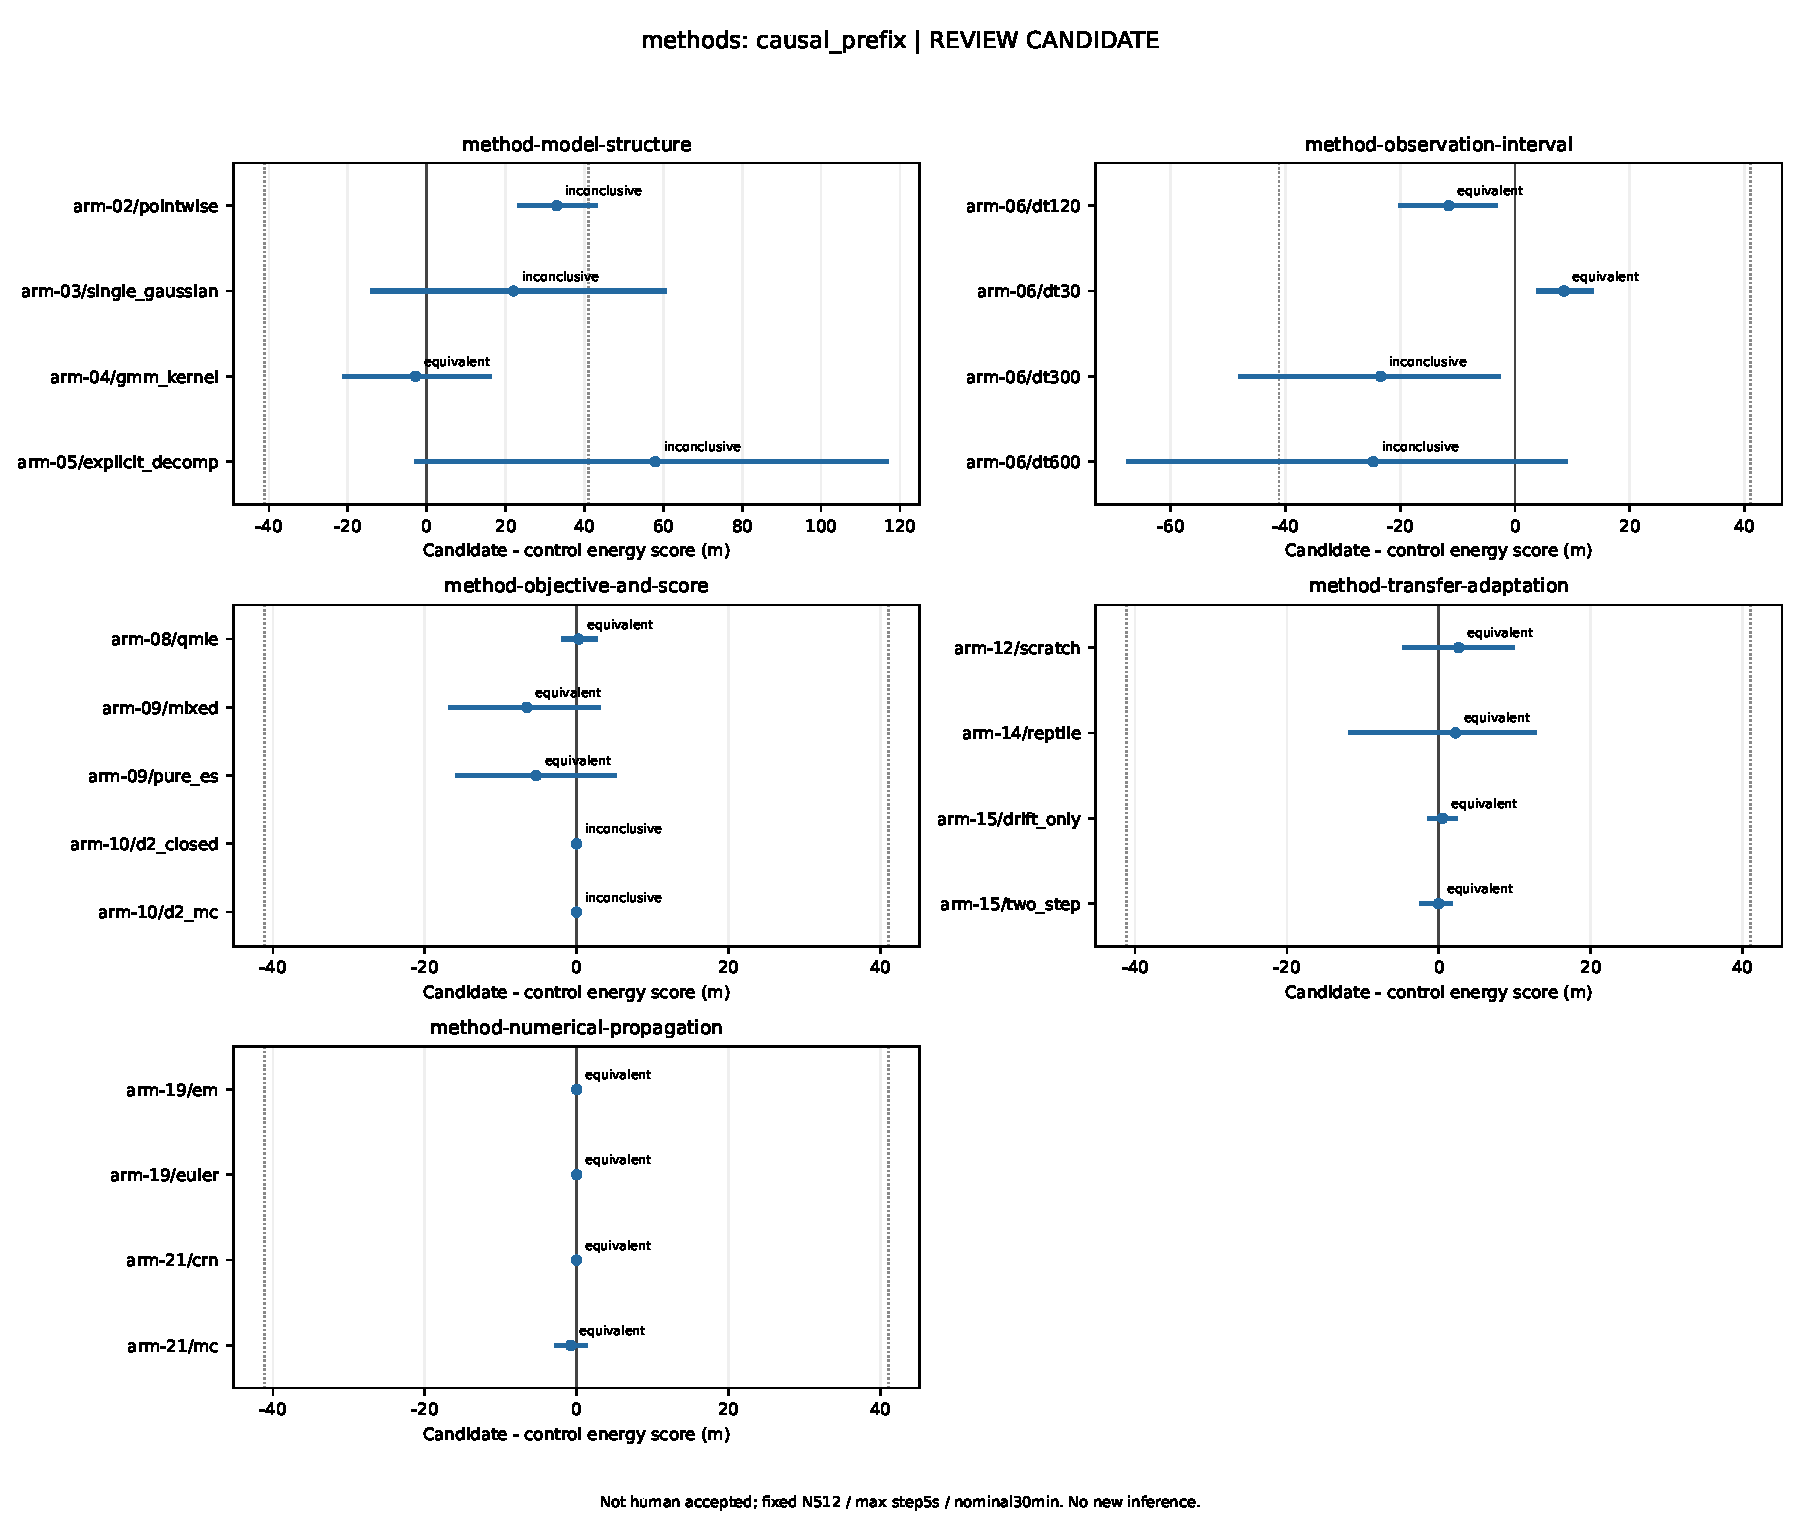
\includegraphics[width=0.96\linewidth,height=0.72\textheight,keepaspectratio]{../final-results-v1/figures/paired-methods-causal_prefix.pdf}
\caption{真实审计绑定的方法主组比较图。保留原分析区间与固定实际意义带。
图中状态是有限算法下的保存判定，不代表分辨率不变资格或已验收科学结论。}
\label{fig:audited-method-comparisons}\hypertarget{fig:audited-method-comparisons}{}
\end{figure}

全部165条原运行时记录现已齐全，其中15条预热不进入延迟分位数，
每个冷／温条件各保留五次试验，30个条件摘要沿用原数值及分母。
宿主中断暴露的时间不扣除、不丢弃。存档运行时图标题
“Isolated cold/warm runtime”仅为历史设计名称，不认证无中断独立延迟或加速；
第~\ref{sec:runtime-environment}节的时钟与中断限制仍适用。

完整匿名卡片、原16份CSV、32张图片及34份双语可选表片段位于
\path{paper/pirc17/final-results-v1/}。
保留所有模式、诊断见证、试验状态及单位。卡片绑定分析
\texttt{d1d67a3b}、审计\texttt{8ff917ad}及导出\texttt{29cb892f}，
完整摘要及文件manifest在结果包内。这是审阅交付，
不等于完整最终论文整合或科学／人工最终验收。
\FloatBarrier



\section{版本与证据绑定}
方法已核对协议
\path{2267ab84fa77ff4039234a61e8f44be1c3713317d8ad2d1bb4ced9af0c5b293a}
及执行身份
\path{c3e44393f6bc5544aaa21bb273c94eaecb9d0becb4e0590771355c4c0be9b6c2}。
原已完成的分析、保存输出审计、公开导出和卡片绑定见
\path{paper/pirc17/final-results-v1/}；后续固定预算算术及卡片引用核对见
\path{paper/pirc17/qualification-v1/}。
完整原匿名输入现已无损公开在 \path{paper/pirc17/replay-input-v1/}。
其中的隔离Python标准库命令可逐字节复算六份CRPS／终点分位数包文件，
不等于全部原配对结论、图表和PDF的公开重建；完整公开路径仍须独立验证，
来源哈希本身不能替代这项证明。
实际算法依据 PIRC-17 直接线性拟合、因果 rollout、评分注册、块推断和卡片模块。
公开稿不包含私密原始数据，并不免除一次独立保存输出复算。


\section{发布与来源对账细节}
\label{sec:source-reconciliation-details}\hypertarget{sec:source-reconciliation-details}{}
以下来源与记账说明保留原报告范围，不新增数据资格检查或实验。
正文仍保留科学人群、输入定义与解释限制。

\paragraph{发布身份与开发分配。}
本次用冻结源函数核对全部 7,618 个文件分配，
并将全部 72,046 个窗口身份连接回文件、记录哈希及划分。
每对发布划分之间的文件、记录哈希、segment 和窗口身份交集均为零。
计数及来源绑定见 \path{paper/pirc17/partition-description-v1.json}。
上述身份核对没有重读原始坐标、速度或时钟数值，因此不是重新计算原始记录哈希、逐点对齐、
参与者独立性或物理时间独立性的审计。

对于 \(n\geq4\) 个点的细分 segment，唯一的 midpoint 样本使用
\(0,\ldots,\max(1,\lfloor n/2\rfloor-1)\) 作为历史索引，紧接其后的目标索引延伸至 \(n-1\)。
全部保存边界满足此规则，窗口身份绑定这些边界，且每个采样 segment 恰有一个窗口。
这排除了该窗口内部历史与目标的索引重叠，不证明不同记录的物理时间或近似路线没有重叠。
训练／适应角色先在完整发布训练样本上划分，再筛选当前任务资格：将其 5,251 个记录块
按字符串 \texttt{20260912:} 加块 ID 的 SHA256 排序，前
\(\operatorname{round}(0.8\times5251)=4201\) 块用于训练，其余 1,050 块用于适应，
分别包含 39,272 与 10,573 个窗口。实际选取的 328 个训练窗口来自 259 块，
76 个适应窗口来自 62 块，81 个验证窗口来自 62 块。
十六个保存方法拟合的原窗口及角色均与该规则一致；完整 release 的窗口数不能替代实际拟合数据量。

\paragraph{评估数据既往使用记录。}
release 报告记载 74 个完全相同的记录哈希组曾跨\emph{旧目录}划分；
这是历史审计报告，不是当前上述零交集划分。
绑定的使用史同时记录：12,370 个窗口的发布最终评估队列此前已被使用。
另一个历史 GeoLife 最终评估集有 17,038 个窗口，但不是本协议队列。
用户在 2026 年 9 月 26 日选择使用已下载数据并保持训练／评估分离，不新建未触碰留出集。
本文保留这个范围，但不将当前评估称为首次使用、对设计完全盲的验证。
协议准备阶段的零读取声明不能抹除历史使用，也不能保证独立确认性质。

\paragraph{保存速率构造。}
保留源构建脚本将输入km/h除以3.6转为m/s，并在源父轨迹的末点复制最后一个区间速率。
该末点填充和上游处理保持原样，不重新生成或修复速率。
同一表的 $v_x,v_y$ 则由局部位置的中心差分构造，端点速度也复制；
其模长不是这里的保存标量，也不使用发布时钟估计新速度。
全部 12,370 个原窗口均有完整、有限、非负的保存标量，统计失败为0；
不移除窗口，也不以成功子集替代任何失败组的分布。

\paragraph{时钟页脚与原发布异常。}
表~\href{supplement.pdf\#tab:clock-use}{科学补充材料} 区分保存时钟与算法时钟。release 将 \texttt{t} 转为
\texttt{datetime64[ns]} 及整数 tick，正式输入加载器核对它与合格来源点的 tick 精确相同。
类型或数值相等检查不是时区及来源认证。按原 condition 清单固定顺序检查前三个文件页脚，
三者字节哈希匹配，均为 \texttt{timestamp[ns]} 且没有时区标注，分别有 951、550、794 行。
这项有限检查不读取逐点数值，也不代表全部 7,618 个文件。
无时区标注的时间戳可能按 UTC 约定保存，但页脚不能证明该约定；本文不据此推断或应用新的时区修正。

原 release 报告记录 37,957 个重复时刻间隔，涉及 1,387 个 segment，
166 个倒退时间切分及 10,052 个超过 60 秒间隔的切分；源 condition 点共 19,647,139 个，
对齐点为 14,738,300 个，未对齐点为 4,908,839 个。
这些是原发布对账总数，不是本次重新计算的逐点结果、时钟误差率或所选 46 个目标的异常数。
R1 清洗、时间细分及资格筛选的分母不同，不能将计数合并为一个错误率。
旧观测适配器 对相同时刻保留首点，并通过选择已有端点平衡历史／目标两侧。
相比之下，正式可见前缀加载器要求保留时刻严格递增，不对新的预测输入静默去重。
元数据、源代码绑定及三个页脚收据见 \path{paper/pirc17/clock-description-v1.json}。

\paragraph{案例地图与模型资产对账。}
私有案例背景使用 WorldCover 2021 v200\cite{worldcover2021}、SRTM 标签的 Skadi 高程\cite{mapzenterrain}、
Overture transportation 2026-08-19.0（包括 OpenStreetMap 与 TomTom 来源）\cite{overture202608,overtureattribution}，
以及 HydroRIVERS v1\cite{hydrorivers2013,hydroriverslicense}。
这些固定地图年代没有被证明与每条来源轨迹同时。
不含路线的 \path{paper/pirc17/map-source-acknowledgements-v1.json} 分别记录
WorldCover 的 CC BY 4.0、交通图层的 ODbL、SRTM 收据声明和 HydroRIVERS 的专属协议，不能给所有图层套同一种许可。
HydroRIVERS 要求的声明和来源引用仍需发表审阅。地图可获得和已有署名不等于有权再分发私密轨迹。
原始路线获取许可、隐私审阅和案例发表授权仍未核实；这里作披露，不宣称已获公开许可。

模型保留的地图目录不同于三份案例背景。表~\href{supplement.pdf\#tab:model-map-catalog}{科学补充材料} 描述五份哈希绑定的
获取收据及冻结特征快照的额外栅格父资产；计数是准入文件，不是实际访问资产、覆盖路线或成功查询数。
1283 个快照父资产与收据目录重叠 1232 个，仅另增 51 个文件；收据原有 1354 个，
合计 1405 个文件也不保证预测位置均有支持。

\paragraph{产品引用与上游来源。}
模型中标为 \texttt{srtm} 的高程通道来自 Mapzen AWS Skadi 分发\cite{mapzenterrain}；
另行准入的 Copernicus 通道为 GLO-30 Public，2021 发布\cite{copernicusdem2021}。
WorldCover v200\cite{worldcover2021}、Overture 2026-08-19.0\cite{overture202608}、
HydroRIVERS v1.0\cite{hydrorivers2013,hydroriverslicense} 标识其余模型输入产品，
不只是案例背景来源。Skadi 格式文档说明该分发使用 SRTM 与其他开放高程来源，
因此收据的 GL1 标签及2000年区间不能认证每份保留瓦片都是纯 NASA SRTM 或具有相同获取年代。
原冻结资产哈希和收据标签保留不变，所引文档版本不作为新指定的数据发布版本。
提供方的署名文档\cite{mapzenattribution,overtureattribution,hydroriverslicense}
与产品引用和方法文献分开；查阅文档不等于完成逐瓦片义务或私密路线发表许可审核。
网页访问日不是下载日或不可变数据版本，缺少逐瓦片上游身份仍是限制。


\section{评分与执行捕获时刻}
\label{sec:score-execution-snapshots}\hypertarget{sec:score-execution-snapshots}{}
2026 年 10 月 6 日 00:54:18.683579 UTC 捕获的评分快照包括登记 11020 项科学预测中的 10384 项成功、
5 项失败及 631 项缺评分。这是捕获时的评分处置，不是实时预测计数。
方法主组全网格完整：28 个配置、46 个记录块及五个预测随机种子，共 6440 行。
每个配置有 230 行，但记录数据单位仍为 46 块。
此次统计没有新增预测、重拟合或重新计算粒子评分。
精确捕获时刻与输入哈希保存在
\path{paper/pirc17/preliminary-method-statistics-v1.json}。
第~\ref{sec:execution-coverage}~节的执行清点于稍后的 06:53:13.846553 UTC 捕获，
成功计数高出 130 项。两者是不同时间的固定快照，不是同时计数；
这里尚未独立审计两快照的逐项差集。

表~\ref{tab:capture-count-difference}~在相同的 114 个配置与起点模式单元上
对账两份保存汇总。计数变化的 22 个单元全部属于地形矩阵：历史前缀、
已知速度、仅位置模式的成功净增分别为 57、8、65 项。
各单元成功计数的增量均等于缺项计数的减量，失败计数不变；
全部 84 个方法单元的计数均不变。
因此，这 130 项计数差没有向方法主组的 6440 行结果表增加观测，
也没有更改其固定输入版本。摘要和方法发现仍对应较早的评分快照，
完整性表仍对应较晚的执行清点。

\begin{table}[htbp]
\centering\small
\caption{保存成功计数的对账，不是逐项预测成员清单的重建。
较早列为 2026 年 10 月 6 日 00:54 的评分汇总，较晚列为同日 06:53 的执行清点。}
\label{tab:capture-count-difference}\hypertarget{tab:capture-count-difference}{}
\begin{tabular}{@{}llrrr@{}}
\toprule
矩阵 & 起点模式 & 较早 & 较晚 & 净增\\
\midrule
方法 & 历史前缀 & 6440 & 6440 & 0\\
方法 & 已知速度 & 838 & 838 & 0\\
方法 & 仅位置 & 840 & 840 & 0\\
地形 & 历史前缀 & 1974 & 2031 & 57\\
地形 & 已知速度 & 292 & 300 & 8\\
地形 & 仅位置 & 0 & 65 & 65\\
\midrule
合计 & & 10384 & 10514 & 130\\
\bottomrule
\end{tabular}
\end{table}

不含路线的 \path{paper/pirc17/capture-count-reconciliation-v1.json}
保存全部单元的两组成功、失败、缺项计数，以及精确捕获时刻和输入文件哈希。
两份原汇总均未保留逐任务工作标识集合，因此净增 130 项不等于已经核验的
130 个新增任务身份；这些计数不能排除同一单元内部的成员替换。
这次计数对账不替代原保存输出独立复算，也不证明内容完整性、独立性或科学资格。
原快照及统计结果均不覆写，未新增预测、评分或重采样。

\clearpage

\section{捕获时预测与比较族完整性}
\label{sec:execution-coverage}\hypertarget{sec:execution-coverage}{}
表~\ref{tab:execution-coverage} 是 2026 年 10 月 6 日 06:53 UTC 捕获的执行清点，
不是新的精度分析。仅读取原任务、预测和评分缓存索引及精确保存来源绑定，不加载预测数组
或重新估计评分。原 11020 项科学预测保留配置、起点模式和五种子分母；捕获时成功
10514 项、可继续运行 501 项、失败 5 项，评分索引数量相同，未发现非法来源绑定。
索引中标为成功并不等于评分内容已独立验证或具有科学结论资格。

\begin{table}[htbp]
\centering\small
\caption{捕获时按矩阵和起点模式清点的独特计划预测；六行合计 11020。模式之间复用块，不是新增受试者。}
\label{tab:execution-coverage}\hypertarget{tab:execution-coverage}{}
\begin{tabular}{@{}llrrrr@{}}
\toprule
矩阵 & 起点模式 & 计划 & 成功 & 可运行 & 失败\\
\midrule
方法 & 因果前缀 & 6440 & 6440 & 0 & 0\\
方法 & 已知速度 & 840 & 838 & 0 & 2\\
方法 & 仅位置 & 840 & 840 & 0 & 0\\
地形 & 因果前缀 & 2300 & 2031 & 266 & 3\\
地形 & 已知速度 & 300 & 300 & 0 & 0\\
地形 & 仅位置 & 300 & 65 & 235 & 0\\
\midrule
合计 & & 11020 & 10514 & 501 & 5\\
\bottomrule
\end{tabular}
\end{table}

第~\href{supplement.pdf\#sec:method-results}{科学补充材料}~节方法结果使用完整 $28\times46\times5=6440$ 主网格，而不是跨矩阵和模式混在一起平均。
已知速度和仅位置均复用前六个主组记录块，只作有界的初始化描述诊断。
已知速度失败分别在 \texttt{single\_gaussian} 与 \texttt{dt30}；地形主组失败分别在
\texttt{all-terrain}、\texttt{lio-road} 和 \texttt{lio-river}。
这些项保留处置，不自动重试，也不从分母删除。

\begin{table}[htbp]
\centering\small
\caption{同一捕获时刻的主比较族必需评分索引行。完整仅指索引齐全；缺失或失败阻止完整配对比较，族之间有重叠。}
\label{tab:family-coverage}\hypertarget{tab:family-coverage}{}
\begin{tabular}{@{}lrrrrl@{}}
\toprule
主比较族 & 必需 & 成功 & 缺失 & 失败 & 处置\\
\midrule
模型结构 & 1150 & 1150 & 0 & 0 & 索引完整\\
观测间隔 & 1150 & 1150 & 0 & 0 & 索引完整\\
目标及评分 & 1380 & 1380 & 0 & 0 & 索引完整\\
训练及适应 & 1150 & 1150 & 0 & 0 & 索引完整\\
数值传播 & 1380 & 1380 & 0 & 0 & 索引完整\\
地形整体／LOO & 1380 & 1219 & 160 & 1 & 不可用\\
地形 LIO & 1150 & 1017 & 131 & 2 & 不可用\\
\bottomrule
\end{tabular}
\end{table}

表~\ref{tab:family-coverage} 按每族独特的必需配置行计数，不是每个对比再增加一组观测。
对照被多个比较族共享，各行不能相加作实验总量。例如两地形族共享 230 行基线；
160 与 131 行缺失中有 25 行共享基线，故主地形独特缺预测为 266 行而非 291 行。
索引齐全不免除独立保存输出审计、机制证据、不确定性检查及最终验收；
失败族不会从成功交集取得效应估计。

501 项待科学预测与原计划的 261 项辅助任务不同：58 条惯性路径、38 次回放、
75 次冷启动计时、15 次排除预热、75 次温启动计时。这些辅助项在捕获时尚未完成，
290 项同网格参考已经完成。预热不计入运行时间测量样本；成本结论必须采用原计时协议，
本清点不代表运行成本。



\Needspace{.70\textheight}

\Needspace{.70\textheight}



\section{CPU 环境详细记录}
\label{sec:runtime-record-details}\hypertarget{sec:runtime-record-details}{}
记录的线程数为 PyTorch 6／inter-op 12，OMP/MKL 6，OpenBLAS/Numba 12；
库线程数不是预测工作进程数。机器描述只给 Intel family/model/stepping，
没有核实营销型号。公开读者投影绑定原环境摘要，排除本机及 DLL 路径。

每项独立 CPU 计时试验携带完整硬件清单的原始摘要，记录平台与处理器报告、逻辑和物理
CPU 数、总内存、Python、NumPy、PyTorch、psutil 版本，以及可用的 DuckDB、Numba、
Rasterio、PyArrow 版本。清单还记录 PyTorch 线程计数、已加载时的 Numba 线程数，以及
OMP、MKL、OpenBLAS、Numba 的线程环境变量。变量未设置不意味着只有一个线程。
公开硬件条目以原始完整清单的摘要为键，省略可能含本机 DLL 路径的已加载原生线程池记录。
最终硬件取值必须来自审计后的计时记录，不能以编译本工作稿的机器代替。
原计时协议中的“温操作系统缓存”措辞不是实测缓存状态保证：试验并未清空、控制或
记录系统缓存占用。原计时收据及其定义保持不变，不重新贴标签或重测。


\section{执行记录与重建}
\label{sec:execution-reconstruction}\hypertarget{sec:execution-reconstruction}{}
继续运行的两路工作处理互不重叠的原始任务身份，各自拥有可变地图查询和历史状态，
由单一派发器原子保存完成记录。30分钟观察记录总成功、失败、剩余及分路增量。
这些是执行观察，不是模型质量评分或额外实验。

闭合保存评分清点与原科学任务元数据在表~\ref{tab:terminal-score-inventory} 的终态计数上一致。
8120项方法预测与2900项地形预测共11020项科学工作；共同评分网格另含290项登记同网格参考
和58条确定性惯性路径，因此是$58\{5(28+10+1)+1\}=11368$个槽位，
不是11368个独立观测。记录块分为46个主要块和12个支持块。
预测失败保留失败评分槽位，不填成零误差。清点不会修复四个不可用比较家族，
也不证明每项评分都与原始输出一致。

\begin{table}[htbp]\centering\small
\caption{2026年10月8日核对的终态保存评分清点。预期数保留全部登记槽位，
成功／失败指保存处置，不是科学资格；参考项不计入11020项科学预测分母。}
\label{tab:terminal-score-inventory}\hypertarget{tab:terminal-score-inventory}{}
\begin{tabular}{@{}lrrr@{}}\toprule
角色 & 预期 & 成功 & 失败\\\midrule
方法预测 & 8120 & 8118 & 2\\
地形预测 & 2900 & 2897 & 3\\
科学预测小计 & 11020 & 11015 & 5\\
同网格参考 & 290 & 290 & 0\\
惯性路径 & 58 & 58 & 0\\
共同评分总计 & 11368 & 11363 & 5\\
\bottomrule\end{tabular}\end{table}

共同评分已闭合全部11368行和58个块，261项原计划辅助试验及独立保存输出复算已完成。
原分析和审计保持不变，公开导出及证据卡片也已生成，不新增预测或拟合，不重复审计。
当前完整审阅结果包见第~\ref{sec:audited-review-update}节。公共消费者已生成十六张表和十六组 PNG/PDF 图，保留原估计、区间、
缺失与单位。登记汇总导出排除原始轨迹、目标、坐标、模型参数和本机路径，记录内容身份与渲染环境，
使复核者可以不重新打开私密数据而重建展示。

复现分为三个不同范围。稿件重建编译指定中英文源文件并解析引用，不重新运行预测。
公共表图重建读取哈希绑定的证据卡片，沿用原始数值和不可用单元，不重新 bootstrap 或检验。
科学复核还需要独立审计保存预测输出及来源绑定。PDF 编译成功不能代替科学审计，也不能
授权实证主张。

最终审核记录需要绑定不可变公开导出和卡片、输入 manifest、协议及执行、渲染库版本和
精确稿件 revision。图的字节一致性仅在登记库和字体环境内成立，不同 TeX 安装不保证
PDF 字节相同。历史稿分开命名，其已有发布工作流不能证明本次 PIRC-17 稿件已获批准或发布。
最终真实署名和验收仍需明确人工决定。



\begin{thebibliography}{99}
\bibitem{johnson2008} D. S. Johnson, J. M. London, M.-A. Lea and J. W. Durban (2008).
Continuous-time correlated random walk model for animal telemetry data.
\emph{Ecology}, 89(5), 1208--1215.
\url{https://doi.org/10.1890/07-1032.1}.
\bibitem{ghahramani2000} Z. Ghahramani and G. E. Hinton (2000).
Variational learning for switching state-space models.
\emph{Neural Computation}, 12(4), 831--864.
\url{https://doi.org/10.1162/089976600300015619}.
\bibitem{avgar2016} T. Avgar, J. R. Potts, M. A. Lewis and M. S. Boyce (2016).
Integrated step selection analysis: bridging the gap between resource selection and animal movement.
\emph{Methods in Ecology and Evolution}, 7(5), 619--630.
\url{https://doi.org/10.1111/2041-210X.12528}.
\bibitem{avgar2017correction} (2017). Corrigendum.
[Correction to Avgar et al.\ (2016)].
\emph{Methods in Ecology and Evolution}, 8(9), 1168.
\url{https://doi.org/10.1111/2041-210X.12725}.
\bibitem{gupta2018} A. Gupta, J. Johnson, L. Fei-Fei, S. Savarese and A. Alahi (2018).
Social GAN: Socially Acceptable Trajectories with Generative Adversarial Networks.
\emph{Proceedings of the IEEE Conference on Computer Vision and Pattern Recognition},
2255--2264.
\url{https://openaccess.thecvf.com/content_cvpr_2018/html/Gupta_Social_GAN_Socially_CVPR_2018_paper.html}.
\bibitem{salzmann2020} T. Salzmann, B. Ivanovic, P. Chakravarty and M. Pavone (2020).
Trajectron++: Dynamically-Feasible Trajectory Forecasting with Heterogeneous Data.
In \emph{Computer Vision -- ECCV 2020}, Lecture Notes in Computer Science,
12363, 683--700. Springer.
\url{https://doi.org/10.1007/978-3-030-58523-5_40}.
\bibitem{kidger2021} P. Kidger, J. Foster, X. Li and T. J. Lyons (2021).
Neural SDEs as Infinite-Dimensional GANs.
\emph{Proceedings of the 38th International Conference on Machine Learning},
Proceedings of Machine Learning Research, 139, 5453--5463.
\url{https://proceedings.mlr.press/v139/kidger21b.html}.
\bibitem{gao2024} T.-T. Gao, B. Barzel and G. Yan (2024).
Learning interpretable dynamics of stochastic complex systems from experimental data.
\emph{Nature Communications}, 15, 6029.
\url{https://doi.org/10.1038/s41467-024-50378-x}.
\bibitem{gneiting2007} T. Gneiting and A. E. Raftery (2007).
Strictly proper scoring rules, prediction, and estimation.
\emph{Journal of the American Statistical Association}, 102(477), 359--378.
\url{https://doi.org/10.1198/016214506000001437}.
\bibitem{gneiting2008} T. Gneiting, L. I. Stanberry, E. P. Grimit,
L. Held and N. A. Johnson (2008). Assessing probabilistic forecasts of
multivariate quantities, with an application to ensemble predictions of
surface winds. \emph{TEST}, 17, 211--235.
\url{https://doi.org/10.1007/s11749-008-0114-x}.
\bibitem{kloeden1992} P. E. Kloeden and E. Platen (1992).
\emph{Numerical Solution of Stochastic Differential Equations}. Springer.
\url{https://doi.org/10.1007/978-3-662-12616-5}.
\bibitem{nichol2018} A. Nichol, J. Achiam and J. Schulman (2018).
On First-Order Meta-Learning Algorithms. [Preprint], \emph{arXiv:1803.02999v3}.
\url{https://arxiv.org/abs/1803.02999v3}.
\bibitem{holm1979} S. Holm (1979).
A simple sequentially rejective multiple test procedure.
\emph{Scandinavian Journal of Statistics}, 6(2), 65--70.
\url{https://www.jstor.org/stable/4615733}.
\bibitem{davison1997} A. C. Davison and D. V. Hinkley (1997).
\emph{Bootstrap Methods and their Application}. Cambridge University Press.
\url{https://doi.org/10.1017/CBO9780511802843}.
\bibitem{noaa} NOAA Global Monitoring Division (n.d.).
\emph{General Solar Position Calculations}. [Online documentation]. Accessed 7 October 2026.
\url{https://gml.noaa.gov/grad/solcalc/solareqns.PDF}.
\bibitem{worldcover2021} D. Zanaga et al. (2022).
\emph{ESA WorldCover 10 m 2021 v200}. [Dataset], version v200.
\url{https://doi.org/10.5281/zenodo.7254221}.
\bibitem{overtureattribution} Overture Maps Foundation (n.d.).
\emph{Attribution and Licensing}. [Online documentation]. Accessed 6 October 2026.
\url{https://docs.overturemaps.org/attribution/}.
\bibitem{hydrorivers2013} B. Lehner and G. Grill (2013).
Global river hydrography and network routing: baseline data and new approaches
to study the world's large river systems.
\emph{Hydrological Processes}, 27(15), 2171--2186.
\url{https://doi.org/10.1002/hyp.9740}.
\bibitem{hydroriverslicense} HydroSHEDS (n.d.).
\emph{HydroRIVERS product documentation and licence}. [Online documentation], version v1.0. Accessed 6 October 2026.
\url{https://www.hydrosheds.org/products/hydrorivers}.
\bibitem{mapzenterrain} Mapzen / Tilezen (2017).
\emph{Terrain Tiles: Types of Terrain Tiles and Skadi format}.
[Dataset distribution documentation]. Document revision e3d4351; accessed 7 October 2026.
\url{https://registry.opendata.aws/terrain-tiles/}.
\url{https://github.com/tilezen/joerd/blob/e3d4351ee3e5be333e23f47cb500e9a7c310656a/docs/formats.md}.
\bibitem{mapzenattribution} Mapzen / Tilezen (2017).
\emph{Terrain Tiles: Attribution}. [Online documentation].
Document revision d8f587b; accessed 7 October 2026.
\url{https://github.com/tilezen/joerd/blob/d8f587b73d26e0a0c42cdccd9ae8c55de4197763/docs/attribution.md}.
\bibitem{copernicusdem2021} Copernicus Programme / Sinergise (2021).
\emph{Copernicus Digital Elevation Model: GLO-30 Public}.
[Dataset distribution documentation], 2021 release; accessed 7 October 2026.
\url{https://registry.opendata.aws/copernicus-dem/}.
\bibitem{overture202608} Overture Maps Foundation (2026).
\emph{2026-08-19 release notes}. [Dataset release documentation].
Data version 2026-08-19.0; accessed 7 October 2026.
\url{https://docs.overturemaps.org/blog/2026/08/19/release-notes/}.
\end{thebibliography}

\end{document}
